\chapter{Durchführung}
\label{ch:durchfuerung}

\section{Versuchsaufbau}

Der Versuchsaufbau besteht aus einem Prismenspektrometer mit zwei hintereinander angeordneten Flintglasprismen, einem beweglichen Spiegel zur Justierung des Lichts auf die Fotozelle, und einem Austrittsspalt, hinter dem sich die Fotokathode befindet. Die Kathode ist über ein Piko-Amperemeter geerdet mit einem Ring verbunden, der als Anode dient. Das Licht einer Hg-Spektrallampe wird auf die Kathode gelenkt. Zur Messung des sehr kleinen Fotostroms fließt dieser durch einen $1\,\text{G}\Omega$-Widerstand, über den eine Spannung proportional zum Strom abfällt. Diese Spannung wird über einen hochohmigen Verstärker um den Faktor 11 verstärkt und als $U_I$ gemessen.

\begin{figure}[!ht]
    \centering
    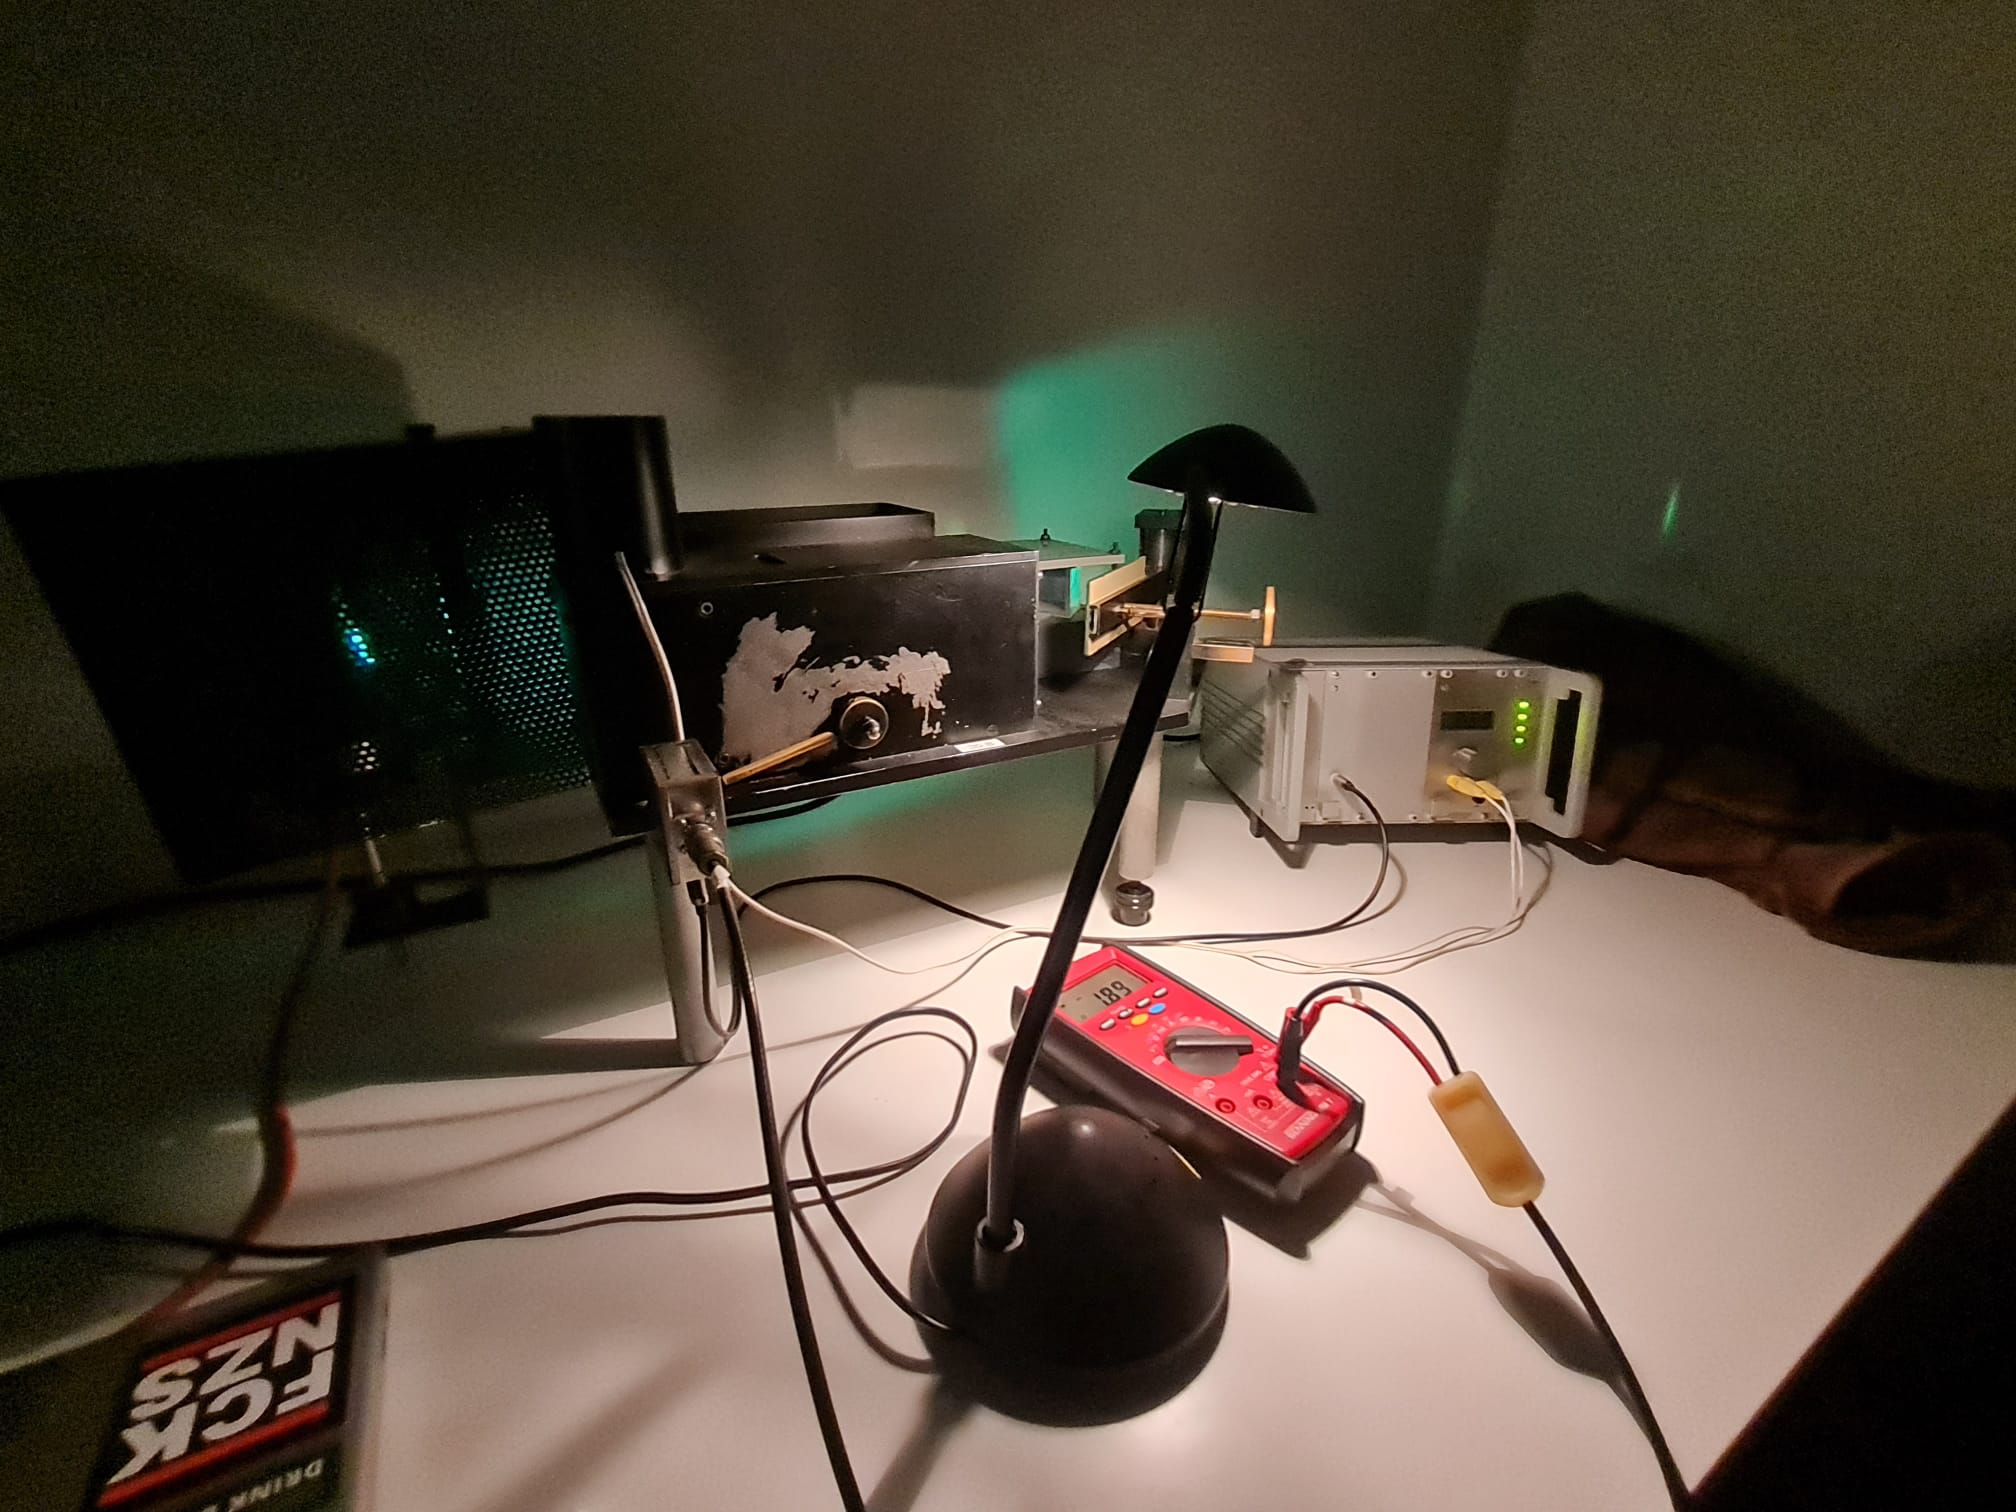
\includegraphics[width=0.3\textwidth]{img/35/va.jpg}
    \caption{Versuchsaufbau}
    \label{fig:v}
\end{figure}

\section{Messverfahren}

\subsection{Messung der Sperrspannungen einzelner Spektrallinien}

Für jede der fünf Spektrallinien (578\,nm, 546\,nm, 436\,nm, 405\,nm, 365\,nm) wird der Spiegel des Spektrometers zunächst grob und anschließend fein justiert, sodass die Linie zentral auf die Fotokathode fällt. Die Vorspannung wird auf 0\,V eingestellt. Danach wird der Fotozellenspiegel aus dem Strahlengang geklappt und die Strom-Spannungskennlinie ab $U=0\,\text{V}$ in Schritten von 0,1\,V bis zu negativ hin aufgenommen. Der Untergrundstrom $U_{I0}$ wird bei -4\,V gemessen.

\subsection{Bestimmung der Sperrspannung}

Aus den aufgenommenen Kennlinien wird der Untergrundstrom abgezogen und die Wurzel des korrigierten Stroms $\sqrt{U_I-U_{I0}}$ gegen die Spannung $U$ aufgetragen. An den linearen Abschnitt der Kurve wird eine Gerade angelegt und der Schnittpunkt mit $I=0$ bestimmt. Dieser Spannung entspricht die Sperrspannung $U_S$ für die jeweilige Linie.

\subsection{Berechnung des Planck'schen Wirkungsquantums}

Die ermittelten Sperrspannungen $U_S$ werden gegen die Frequenzen $f$ der jeweiligen Spektrallinien aufgetragen. Nach Gleichung \hyperref[eq:sperrspannung]{Gleichung \ref*{eq:sperrspannung}} entspricht die Steigung der linearen Ausgleichsgeraden dem Quotienten $h/e$, wodurch $h$ berechnet werden kann.

\begin{figure}[!ht]
    \centering
    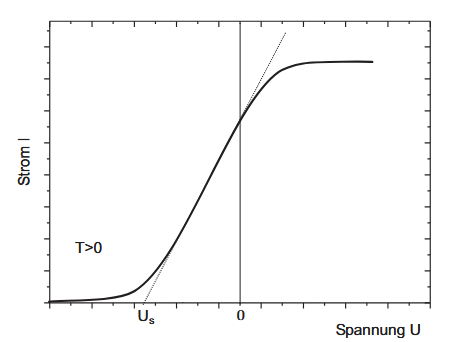
\includegraphics[width=0.3\textwidth]{img/35/gr.png}
    \caption{Strom-Spannungskennlinie einer realen Fotozelle.}
    \label{fig:v}
\end{figure}